\documentclass[
  bibliography=totoc,     % Literatur im Inhaltsverzeichnis
  captions=tableheading,  % Tabellenüberschriften
  titlepage=firstiscover, % Titelseite ist Deckblatt
]{scrartcl}

% Paket float verbessern
\usepackage{scrhack}

% Warnung, falls nochmal kompiliert werden muss
\usepackage[aux]{rerunfilecheck}

% unverzichtbare Mathe-Befehle
\usepackage{amsmath}
% viele Mathe-Symbole
\usepackage{amssymb}
% Erweiterungen für amsmath
\usepackage{mathtools}

% Fonteinstellungen
\usepackage{fontspec}
% Latin Modern Fonts werden automatisch geladen
% Alternativ zum Beispiel:
%\setromanfont{Libertinus Serif}
%\setsansfont{Libertinus Sans}
%\setmonofont{Libertinus Mono}

% Wenn man andere Schriftarten gesetzt hat,
% sollte man das Seiten-Layout neu berechnen lassen
\recalctypearea{}

% deutsche Spracheinstellungen
\usepackage{polyglossia}
\setmainlanguage{german}


\usepackage[
  math-style=ISO,    % ┐
  bold-style=ISO,    % │
  sans-style=italic, % │ ISO-Standard folgen
  nabla=upright,     % │
  partial=upright,   % ┘
  warnings-off={           % ┐
    mathtools-colon,       % │ unnötige Warnungen ausschalten
    mathtools-overbracket, % │
  },                       % ┘
]{unicode-math}

% traditionelle Fonts für Mathematik
\setmathfont{Latin Modern Math}
% Alternativ zum Beispiel:
%\setmathfont{Libertinus Math}

\setmathfont{XITS Math}[range={scr, bfscr}]
\setmathfont{XITS Math}[range={cal, bfcal}, StylisticSet=1]

% Zahlen und Einheiten
\usepackage[
  locale=DE,                   % deutsche Einstellungen
  separate-uncertainty=true,   % immer Fehler mit \pm
  per-mode=symbol-or-fraction, % / in inline math, fraction in display math
]{siunitx}

% chemische Formeln
\usepackage[
  version=4,
  math-greek=default, % ┐ mit unicode-math zusammenarbeiten
  text-greek=default, % ┘
]{mhchem}

% richtige Anführungszeichen
\usepackage[autostyle]{csquotes}

% schöne Brüche im Text
\usepackage{xfrac}

% Standardplatzierung für Floats einstellen
\usepackage{float}
\floatplacement{figure}{htbp}
\floatplacement{table}{htbp}

% Floats innerhalb einer Section halten
\usepackage[
  section, % Floats innerhalb der Section halten
  below,   % unterhalb der Section aber auf der selben Seite ist ok
]{placeins}

% Seite drehen für breite Tabellen: landscape Umgebung
\usepackage{pdflscape}

% Captions schöner machen.
\usepackage[
  labelfont=bf,        % Tabelle x: Abbildung y: ist jetzt fett
  font=small,          % Schrift etwas kleiner als Dokument
  width=0.9\textwidth, % maximale Breite einer Caption schmaler
]{caption}
% subfigure, subtable, subref
\usepackage{subcaption}

% Grafiken können eingebunden werden
\usepackage{graphicx}
% größere Variation von Dateinamen möglich
\usepackage{grffile}

% schöne Tabellen
\usepackage{booktabs}

% Verbesserungen am Schriftbild
\usepackage{microtype}

% Literaturverzeichnis
\usepackage[
  backend=biber,
]{biblatex}
% Quellendatenbank
\addbibresource{lit.bib}
\addbibresource{programme.bib}

% Hyperlinks im Dokument
\usepackage[
  unicode,        % Unicode in PDF-Attributen erlauben
  pdfusetitle,    % Titel, Autoren und Datum als PDF-Attribute
  pdfcreator={},  % ┐ PDF-Attribute säubern
  pdfproducer={}, % ┘
]{hyperref}
% erweiterte Bookmarks im PDF
\usepackage{bookmark}

% Trennung von Wörtern mit Strichen
\usepackage[shortcuts]{extdash}

\author{%
  AUTOR A\\%
  \href{mailto:authorA@udo.edu}{authorA@udo.edu}%
  \texorpdfstring{\and}{,}%
  AUTOR B\\%
  \href{mailto:authorB@udo.edu}{authorB@udo.edu}%
}
\publishers{TU Dortmund – Fakultät Physik}


\subject{V703}
\title{Das Geiger-Müller-Zälrohr}

\date{
  \begin{align}
    \text{Durchführung: } & \text{17.4.2018} & \hspace{3em} & \text{Abgabe: 24.4.2018} \notag
%\\  \text{Korrektur: } & \text{24.4.2018} & \hspace {3em} & \notag
  \end{align}
}

%\date{%
%  Durchführung: DATUM
%  \hspace{3em}
%  Abgabe: DATUM
%}

\begin{document}

\maketitle
\thispagestyle{empty}
\tableofcontents
\newpage

\section{Theorie}
\label{sec:Theorie}
Das Geiger-Müller-Zählrohr ist eines der wichtigsten Messgeräte für ionisierende Strahlung,
insbesondere $\alpha$- und $\beta$-Strahlung, welche zu fast \SI{100}{\percent} detektiert wird.
$\gamma$-Strahlung wird nur zu etwa \SI{1}{\percent} aufgenommen,
sodass nur hohe Intensitäten mit diesem Versuchsaufbau gemessen werden sollten.

Für jedes in seinem Inneren absorbierten Teilchen erzeugt es einen elektronischen Impuls,
der anschließend durch einen Impulszähler aufgenommen wird.
Somit kann die Intensität der Strahlung bestimmt werden.

\subsection{Aufbau des Geiger-Müller-Zählrohrs}
Das Geiger-Müller-Zählrohr besteht im Wesentlichen aus einer zylindrischen Kathode in welcher ein Anodendraht positioniert ist.
Die Kathode besitzt an einer Seite ein Eintrittsfenster, durch welches die Strahlung nahezu ungehemmt eintreten kann.
Zwischen Kathode und Anode ist ein spezielles Gasgemisch unter niedrigem Druck eingefüllt.
Zwischen den Elektroden wird eine Spannung in der Größenordnung $\SI{100}{\volt}$ bis $\SI{1000}{\volt}$ angelegt.

\subsection{Funktion}
Wenn nun eines der Gasmoleküle innerhalb des Zählrohrs durch Strahlung ionisiert wird, wird das ausgelöste Elektron Richtung Anode und das ionisierte Molekül
Richtung Kathode beschleunigt. Dabei wird das Elektron so stark beschleunigt, dass es wiederum weitere Moleküle ionisieren kann.
Es kommt außerdem durch Stoßprozesse zur Erzeugung von UV-Strahlung, sodass sich die Kettenreaktion der Ladungsauslösung
auch senkrecht zum E-Feld, und somit durch das gesamte Zählrohr, ausbreiten kann.

Dies hat den Vorteil, dass dadurch so große Impulse entstehen, dass sie nicht besonders stark verstärkt werden müssen und die
Messung vergleichsweise einfach ist. Ein Nachteil ist jedoch, dass die Messung keine Information
über die Energie der Strahlung hergibt. Somit kann auch nicht mehr zwischen $\alpha$-, $\beta$- und $\gamma$-Strahlung unterschieden werden.

Ionen benötigen wesentlich länger als Elektronen, um die Kathode zu erreichen.
Das bewirkt unter Anderem, dass die Entladungslawinen nicht unbegrenz lange stattfinden, da die effektive Feldstärke
im Zählrohr abnimmt.
In diesem Zustand sind keine weiteren Ionisationen durch eingehende Strahlung mehr möglich.
Die Zeit, in der nach einem registrierten Event keine neuen Events aufgenommen werden können, wird Totzeit genannt.
Nach der Totzeit folgt ein Bereich, die Erholungszeit, in dem die erzeugten Impulse schwächer sind als zuvor.

Die Zeit, die ein Ion bis zur Zylinderwand braucht, ist in der Regel länger als die Totzeit, sodass der Effekt nicht von neuen
Strahlungsevents unterschieden werden kann und die Messung stark verfälscht.
Daher liegt ein besonderes Augenmerk auf der Vermeidung der sogenannten Nachentladungen.

Um zu verhindern, dass die Ionen, welche durch das Feld beschleunigt werden, weitere Elektronen ausschlagen,
wenn sie die Kathode erreichen, werden dem Gas vielatomige Moleküle mit vielen Schwingungsmoden zugefügt. Diese geben eines ihrer Elektronen an die Ionen ab
und werden statt ihrer zur Kathodenwand beschleunigt.
Dort können sie jedoch kein Elektron ausschlagen, sondern werden nur zu Schwingungen angeregt.

\subsection{Kenngrößen}
Wird die Anzahl der gemessenen Events $N$ gegen die am Zählrohr angelegte Spannung aufgetragen, so ergibt sich die Charakteristik
des Zählrohrs, beispielhaft in Abbildung \ref{fig:plateau}.
\begin{figure}[H]
  \centering
  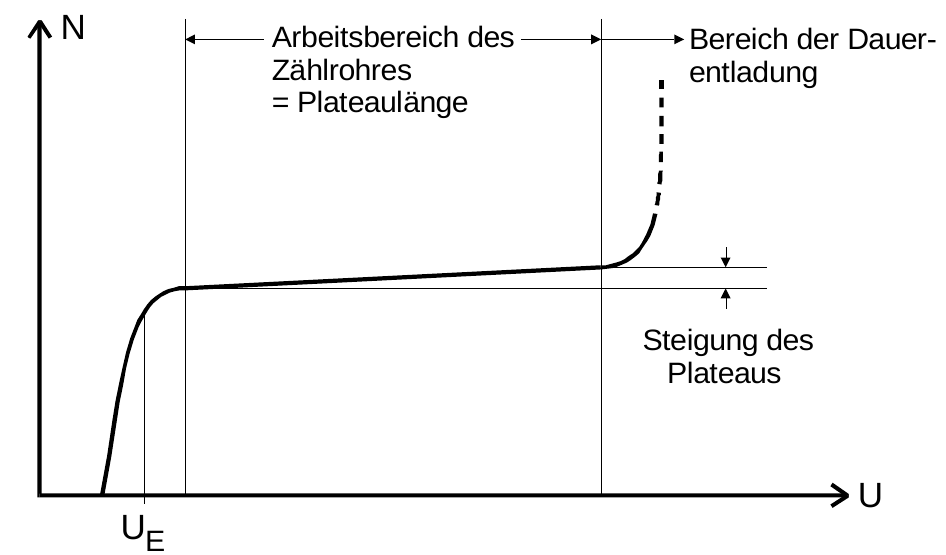
\includegraphics[width=\textwidth]{content/plateau.png}
  \caption{Charakeristik des Zählrohrs.\cite{v703}}
  \label{fig:plateau}
\end{figure}
Der lineare Teil der Chakateristik wird Plateau genannt.
Im wesentlichen wird die Steigung dieser bestimmt durch die Anzahl der Nachentladungen.
Je flacher das Plateau, das heißt je weniger die Anzahl der Events von der Spannung abhängen, desto besser ist das Zählrohr.

Die Totzeit lässt sich durch die Zwei-Quellen-Methode und über eine oszillographische Messung bestimmen.
Für die oszillographische Messung wird das Zählrohr an ein Oszilloskop angeschlossen.
Es wird für eine hohe Strahlenintensität gesorgt.
Auf dem Oszilloskop sollte ein Bild gemäß Abbildung \ref{fig:osz} erscheinen.
\begin{figure}[H]
  \centering
  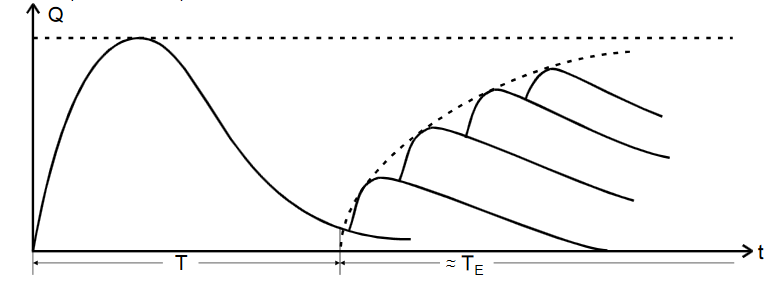
\includegraphics[width=\textwidth]{content/Totzeit.png}
  \caption{Tot- und Erholungszeit im Ladungs-Zeit-Diagramm.\cite{v703}}
  \label{fig:osz}
\end{figure}

Bei bekannter Ablenkgeschwindigkeit kann dann aus dem Bild die Totzeit abgeschätzt werden.
Bei der Zwei-Quellen-Methode wird zunächst ein Strahler mit dem Zählrohr vermessen. Anschließend wird ein zusätzlich ein zweiter Strahler
auf das Zählrohr gerichtet und die Messung wiederholt.
Zu guter letzt wird der erste Strahler entfernt und die Messung ein drittes mal durchgeführt.
Aus simpler Überlegung folgt für die gemessene Rate $N_\text{mess}$, die eigentliche Rate $N$ und die Totzeit $T$ allgemein:
\begin{equation}
    N = \frac{N_\text{mess}}{1-TN_\text{mess}}
\end{equation}
Und somit erhält man hier:
\begin{align}
    N_1     &= \frac{N_{1,\text{mess}}}{1-TN_{1,\text{mess}}} \\
    N_2     &= \frac{N_{2,\text{mess}}}{1-TN_{2,\text{mess}}}
\end{align}
\begin{align}
    N_{1+2} &= \frac{N_{1+2,\text{mess}}}{1-TN_{1+2,\text{mess}}} \\
            &= N_1 + N_2 \\
    \frac{N_{1+2,\text{mess}}}{1-TN_{1+2,\text{mess}}} &=\frac{N_{1,\text{mess}}}{1-TN_{1,\text{mess}}} + \frac{N_{2,\text{mess}}}{1-TN_{2,\text{mess}}}
\end{align}
Es ergibt sich für die Totzeit T näherungsweise:
\begin{equation}
    \label{eqn:totzeit}
    T \approx \frac{N_{1,\text{mess}} + N_{2,\text{mess}} - N_{1+2,\text{mess}}}{2N_{1,\text{mess}}N_{2,\text{mess}}}
\end{equation}

Die pro Event freigesetzte Ladung lässt sich über den mittleren Strom bestimmen.
Hierzu wird folgende Gleichung verwendet:
\begin{equation}
    \overline{I} = \frac{\symup{\Delta}Q}{\symup{\Delta}t} = \frac{\symup{\Delta}q N_\text{mess}}{\symup{\Delta}t}
\end{equation}
Somit folgt:
\begin{equation}
    \label{eqn:ladung}
    \symup{\Delta}q = \frac{\overline{I} \symup{\Delta} t}{N_\text{mess}}
\end{equation}
%\cite{sample}

\section{Durchführung}
\label{sec:Durchführung}
Der Veruch wird gemäß Abbildung\ref{fig:aufb} aufgebaut.
\begin{figure}[H]
  \centering
  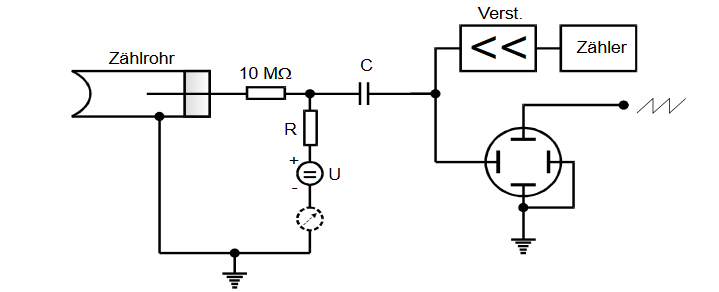
\includegraphics[scale=0.4]{content/Aufbau.png}
  \caption{Versuchsaufbau.}
  \label{fig:aufb}
\end{figure}

\subsection{Aufnahme der Charakteristik des Zählrohrs}
Der Strahlengang eines $\beta$-Strahlers wird auf das Zählrohr ausgerichtet.
Die Messung wird mit einer Anliegenden Spannung $U= \SI{300}{\volt}$ begonnen.
Die Aktivität wird für $\SI{60}{\second}$ aufgenommen.
Zusätzlich wird mit einem empfindlichen Strommessgerät der Zählerstrom gemessen und über die Messzeit gemittelt.
Die Anliegende Spannung wird nach jeder so erfolgten Messung um $\SI{10}{\volt}$ erhöht bis eine Spannung von $\SI{700}{\volt}$ erreicht wird.
\subsection{Oszillographische Messung der Totzeit}
Das Zählrohr wird an ein Oszilloskop angeschlossen.
Die Zählrohrspannung wird auf $\SI{700}{\volt}$ hochgestellt.
Aus dem so enstantendem Bild wird die Totzeit und die Erholungszeit abgelesen.
\subsection{Bestimmung der Totzeit mit der Zwei-Quellen-Methode}
Die Zählrohrspannung wird auf $500$ Volt geschaltet.
Die Aktivität des ausgerichteten Strahlers wird für $\SI{60}{\second}$ gemessen.
Ein zweiter, schwächerer, $\beta$-Strahler wird auf  das Zählrohr ausgerichtet.
Erneut wird die Aktivität für $\SI{60}{\second}$ gemessen.
Der erste $\beta$-Strahler wird entfernt und die Aktivität des zweiten Strahlers wird nach gleichem Verfahren gemessen.

\section{Auswertung}
\label{sec:Auswertung}
\subsection{Bestimmung der Charakteristik des Geiger-Müller-Zählrohrs}
Die durch die Messung erhaltenen Messwerte sind in der Tabelle\ref{tab:mess} aufgetragen.
\begin{table}
    \centering
    \caption{Spannung, Aktivität des $\beta$-Strahlers und Zählerstrom.}
    \label{tab:mess}
    \begin{tabular}{S[table-format=3.0] S[table-format=5.0] S[table-format=1.2(0)e0]}
        \toprule
        {$U/\si{\volt}$} & {Counts} & {$I/\si{\micro\ampere}$}  \\
        \midrule
        320 & 13914 & 0.2 \\
        330 & 14186 & 0.3 \\
        340 & 14550 & 0.3 \\
        350 & 14414 & 0.4 \\
        360 & 14448 & 0.4 \\
        370 & 14703 & 0.5 \\
        380 & 14753 & 0.5 \\
        390 & 14587 & 0.6 \\
        400 & 14662 & 0.6 \\
        410 & 14819 & 0.7 \\
        420 & 14822 & 0.7 \\
        430 & 14820 & 0.8 \\
        440 & 15033 & 0.9 \\
        450 & 14903 & 0.95 \\
        460 & 15125 & 1.0 \\
        470 & 15013 & 1.0 \\
        480 & 15076 & 1.1 \\
        490 & 14963 & 1.1 \\
        500 & 14790 & 1.2 \\
        510 & 15127 & 1.2 \\
        520 & 15237 & 1.3 \\
        530 & 15098 & 1.4 \\
        540 & 15076 & 1.4 \\
        550 & 15163 & 1.45 \\
        560 & 14876 & 1.5 \\
        570 & 15207 & 1.6 \\
        580 & 15064 & 1.6 \\
        590 & 15124 & 1.7 \\
        600 & 15097 & 1.7 \\
        610 & 15080 & 1.8 \\
        620 & 15113 & 1.8 \\
        630 & 15356 & 1.9 \\
        640 & 15473 & 2.0 \\
        650 & 15406 & 2.0 \\
        660 & 15472 & 2.1 \\
        670 & 15856 & 2.1 \\
        680 & 16136 & 2.2 \\
        690 & 16534 & 2.3 \\
        700 & 17078 & 2.4 \\
        \bottomrule
    \end{tabular}
\end{table}
\noindent Die Aufgenommenen Zählraten sind Poissonverteilt, daher ergibt sich ihre Unsicherheit wie folgt:
\begin{equation}
  \sigma = \sqrt{N}
\end{equation}
Die Messwerte sind in Abbildung\ref{fig:plot} aufgetragen und es wurde eine lineare Ausgleichsgerade durch diese gezogen.
\begin{figure}[H]
  \centering
  \includegraphics{build/messung1.pdf}
  \caption{Charakeristik des Zählrohrs.}
  \label{fig:plot}
\end{figure}
\noindent  Die Ausgleichsgerade wurde mit Python/SciPy mit der Funktion $f(x)= Ax + B$ erstellt.
Damit erfolgt eine Steigung von
\begin{equation}
  A = \SI{0.071 \pm 0.008}{\becquerel\per\volt}
\end{equation}
und ein $y$-Achsenabchnitt von
\begin{equation}
  B =   \SI[per-mode=reciprocal]{215\pm 4}{\volt}        .
\end{equation}
\subsection{Oszillographische Messung der Totzeit}
Mit der beschriebenen Messung konnte eine Totzeit von ungefähr
\begin{equation*}
  t_\text{tot} = \SI{70}{\micro \second}
\end{equation*}
und eine Erholungszeit von ungefähr
\begin{equation*}
    t_\text{erhol} = \SI{225}{\micro\second}
\end{equation*}
bestimmt werden.
\subsection{Bestimmung der Totzeit mit der Zwei-Quellen-Methode}
Die erhaltenen Messwerte sind in Tabelle\ref{tab:2strahl} aufgetragen.
\begin{table}[H]
  \caption{Gemessene Werte für die Zwei-Quellen-Methode.}
  \label{tab:2strahl}
  \centering
  \sisetup{table-format=5.3(4)}
  \begin{tabular}{c S[table-format=5.0(0)] S}
    \toprule
    {Quelle} & {Counts} & {Aktivität$/\si{\becquerel}$}\\
    \midrule
    {$N_1$}     & 14440 & 240.667\pm2.003  \\
    {$N_{1+2}$} & 14987 & 249.783\pm2.040  \\
    {$N_2$}     & 614   & 10.233 \pm0.413  \\
    \bottomrule
  \end{tabular}
\end{table}
Damit lässt sich die Totzeit mit Gleichung auf
\begin{equation*}
  T=
\end{equation*}
abschätzen.
Der Fehler berechnet sich hier nach Gauß mit:
\begin{equation}
  \symup{\Delta} T =
\end{equation}
%
\subsection{Bestimmung der mittleren Ladung pro Event}
Die Ladung wird gemäß Formel \eqref{eqn:ladung} berechnet und ist gegen die entsprechende Spannung in 
Tabelle \ref{tab:ladung} aufgetragen.
\begin{table}
    \centering
    \caption{Spannung und Landung pro Event.}
    \label{tab:ladung}
    \begin{tabular}{S[table-format=3.0] S[table-format=2.2e2]}
        \toprule
        {$U/\si{\volt}$} & {$\symup{\Delta}q/e$}  \\
        \midrule
320 &    5.38e12\\
330 &    7.92e12\\
340 &    7.72e12\\
350 &    10.39e12\\
360 &    10.37e12\\
370 &    12.74e12\\
380 &    12.69e12\\
390 &    15.41e12\\
400 &    15.33e12\\
410 &    17.69e12\\
420 &    17.69e12\\
430 &    20.22e12\\
440 &    22.42e12\\
450 &    23.87e12\\
460 &    24.76e12\\
470 &    24.95e12\\
480 &    27.33e12\\
490 &    27.53e12\\
500 &    30.39e12\\
510 &    29.71e12\\
520 &    31.95e12\\
530 &    34.73e12\\
540 &    34.78e12\\
550 &    35.82e12\\
560 &    37.77e12\\
570 &    39.41e12\\
580 &    39.78e12\\
590 &    42.10e12\\
600 &    42.17e12\\
610 &    44.71e12\\
620 &    44.61e12\\
630 &    46.34e12\\
640 &    48.41e12\\
650 &    48.62e12\\
660 &    50.83e12\\
670 &    49.60e12\\
680 &    51.06e12\\
690 &    52.10e12\\
700 &    52.63e12\\
        \bottomrule
    \end{tabular}
\end{table}

\section{Diskussion}
\label{sec:Diskussion}
In guter näherung lässt sich ein Plateau für die Charakterristik des Geiger-Müller-Zählrohrs erkennen.
Die große Differenz der bestimmten Totzeiten lässt sich zum einen damit erklären, dass beide Methoden lediglich eine Abschätzung sind und keine genauen Werte versprechen.
Andereseits konnte, durch die Eichung des Oszilloskops der Wert stark verändert werden, somit ist die Aussagekraft dieses Wertes stark anzuzweifeln.
Anhand von Tabelle \ref{tab:ladung} lässt sich erkennen, dass die Ladungsmenge mit der anliegenden Spannung ansteigt.
Es kommen Ladungen mit dem Faktor $\num{10e12}$ im Zählrohr an.
Anhand der großen Anzahl lässt sich folgern, dass es sich nicht um lokale Entladungen handelt sondern diese im ganzen Zählrohr stattfinden.
  


\nocite{*}
\printbibliography{}

\end{document}
